\chapter{Exercise 05}
\extitle{Let’s Make Nice Plots}
\turnindir{ex05}
\exnumber{05}
\exfiles{plot.py}
\exforbidden{None}
\makeheaderfilesforbidden

\info{
For your information, the task we are performing here is called \textbf{regression}.
It means that we are trying to predict a continuous numerical attribute for all examples (like a price, for instance).
Later in the bootcamp, you will see that we can predict other things such as categories.
}

% ================================= %
\section*{Objective}
% --------------------------------- %
You must implement a function to plot the data and the prediction line (or regression line).\\
\newline
You will plot the data points (with their x and y values), and the prediction line that represents your hypothesis ($h_{\theta}$).
\newpage
% ================================= %
\section*{Instructions}
% --------------------------------- %
In the plot.py file, create the following function as per the instructions given below:

\begin{minted}[bgcolor=darcula-back,formatcom=\color{lightgrey},fontsize=\scriptsize]{python}
def plot(x, y, theta):
    """Plot the data and prediction line from three non-empty numpy.array.
    Args:
      x: has to be an numpy.array, a one-dimensional array of size m.
      y: has to be an numpy.array, a one-dimensional array of size m.
      theta: has to be an numpy.array, a two-dimensional array of shape 2 * 1.
    Returns:
        Nothing.
    Raises:
      This function should not raise any Exceptions.
    """
    ... Your code ...
\end{minted}

% ================================= %
\section*{Examples}
% --------------------------------- %

\begin{minted}[bgcolor=darcula-back,formatcom=\color{lightgrey},fontsize=\scriptsize]{python}
import numpy as np
x = np.arange(1,6)
y = np.array([3.74013816, 3.61473236, 4.57655287, 4.66793434, 5.95585554])

# Example 1:
theta1 = np.array([[4.5],[-0.2]])
plot(x, y, theta1)
# Output:
\end{minted}

\begin{figure}[H]
  \centering
  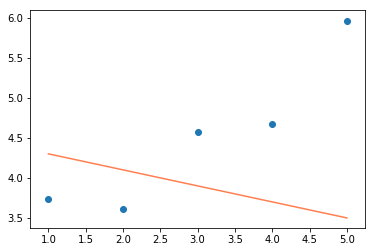
\includegraphics[scale=0.6]{assets/plot1.png}
\end{figure}

\newpage

\begin{minted}[bgcolor=darcula-back,formatcom=\color{lightgrey},fontsize=\scriptsize]{python}
# Example 2:
theta2 = np.array([[-1.5],[2]])
plot(x, y, theta2)
# Output:
\end{minted}

\begin{figure}[H]
  \centering
  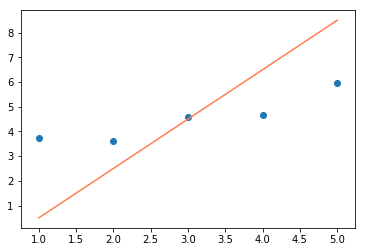
\includegraphics[scale=0.6]{assets/plot2.png}
  \caption{Example 2}
\end{figure}

\begin{minted}[bgcolor=darcula-back,formatcom=\color{lightgrey},fontsize=\scriptsize]{python}
# Example 3:
theta3 = np.array([[3],[0.3]])
plot(x, y, theta3)
# Output:
\end{minted}

\begin{figure}[H]
  \centering
  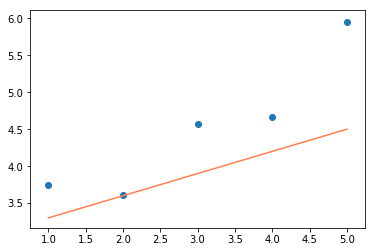
\includegraphics[scale=0.6]{assets/plot3.png}
  \caption{Example 3}
\end{figure}

